%----------------------------------------------------------------------------
\chapter{Design and implementation}
\label{chap:designimplementation}
%----------------------------------------------------------------------------

Let's recap the task flow of the task I described in the Introduction: After
configuring the simulator with the designed camera setting I render multiple
traffic scenarios in different maps provided by CARLA while extracting all
necessary information into a log file to later compare the detection log with


\begin{figure}[!ht]
    \centering
    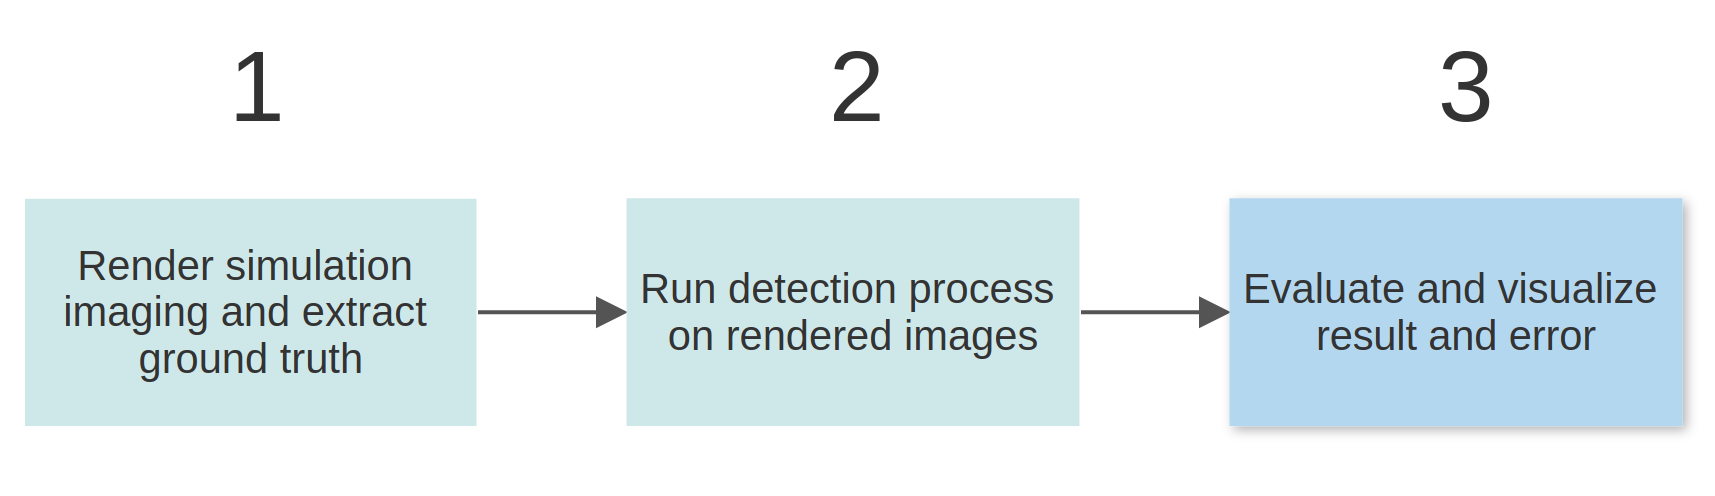
\includegraphics[width=150mm, keepaspectratio]{figures/flowchart.png}
    \caption{Task flow}
    \label{fig:flow2}
\end{figure}


\section{Tools used}

Very soon it became obvious that a Linux operating system is the right way to
develop everything. I have been using Ubuntu before this project as well so I
was already familiar with everything. The main IDE I used throughout the project
is Visual Studio Code, which thanks to it's openness and community has a lot of
extensions that helped me develop in fact every part of the thesis: Python,
Nodejs and Javascript for the webvisualizer and finally LaTeX and ofcourse git
support.

- VS Code
- Python, Scripts, Conda, Jupyter

\section{Choosing the sensor suite}

Mounting cameras around the vehicle to have an all around vision is an essential
design strategy, as we have seen in the work of other companies in
\autoref{chap:relatedwork}. However we will need to determine depth as well. I
decided to use only cameras in a stereoscopic structure to create 4 stereo sides
around the vehicle. The following model shows the design setting \refstruc{fig:3dmodel3}.

\begin{figure}[!ht]
    \centering
    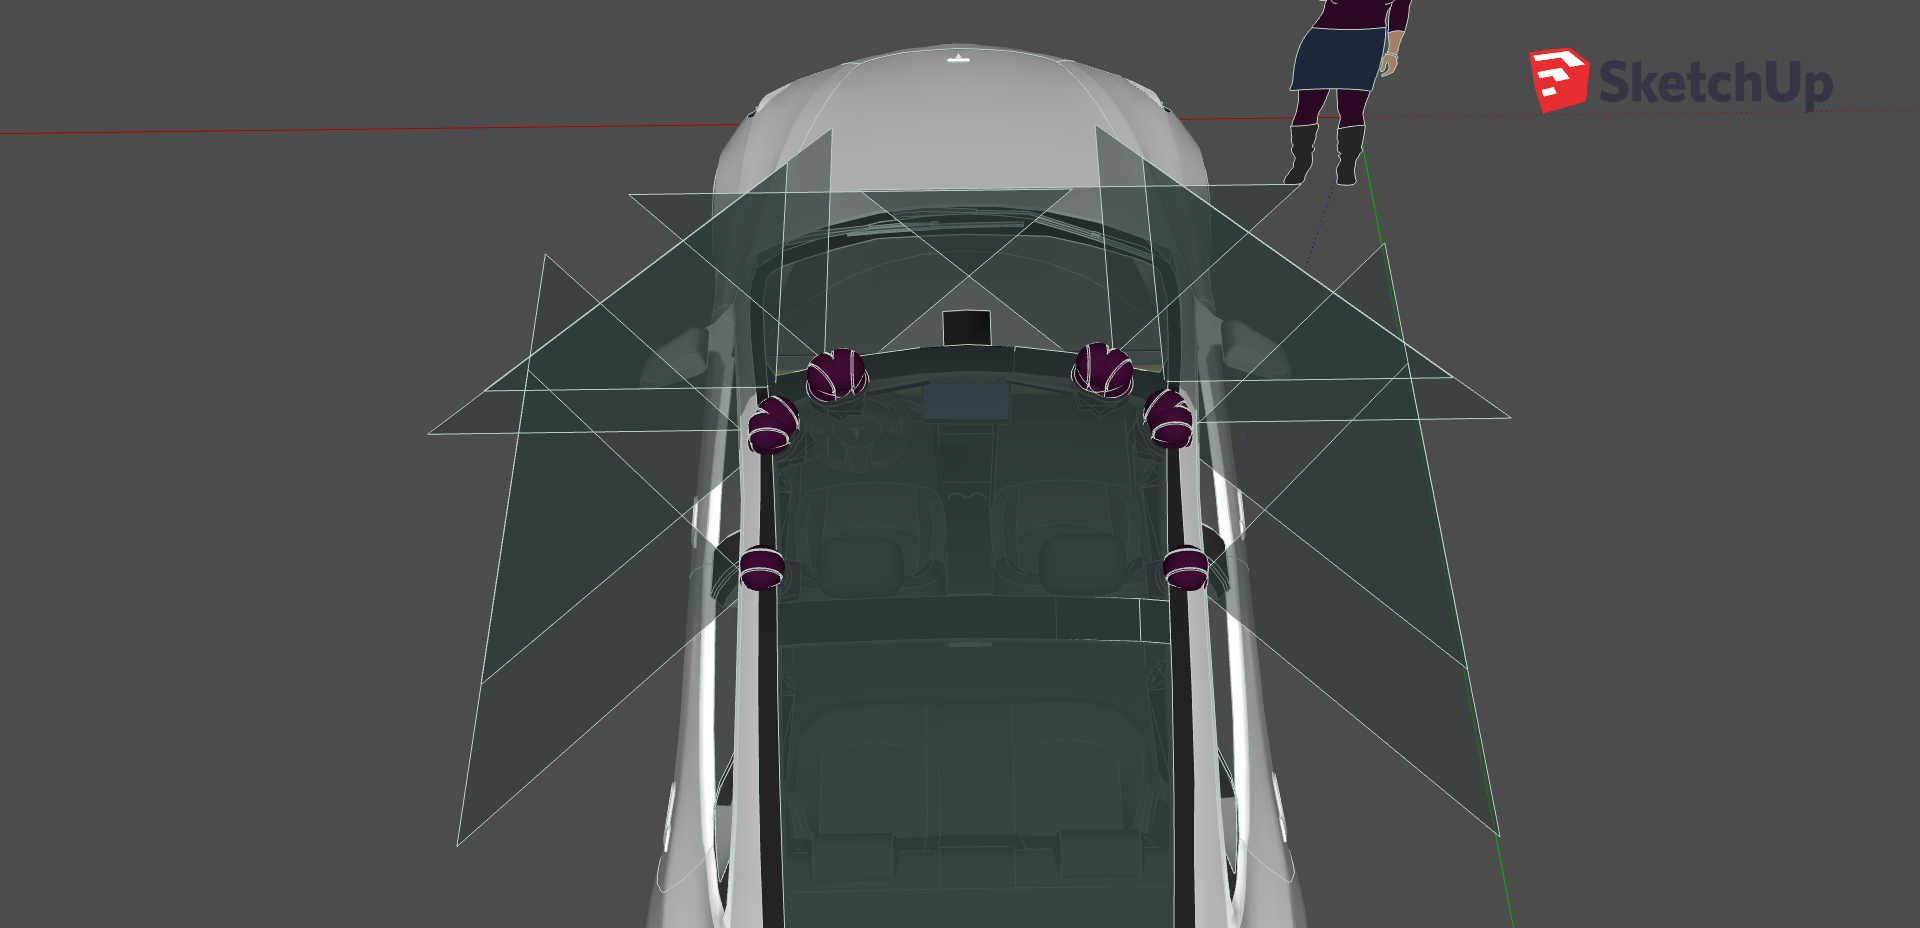
\includegraphics[width=150mm, keepaspectratio]{figures/3dmodel3.png}
    \caption{The stereo camera setting I used on top of the virtual Tesla Model 3}
    \label{fig:3dmodel3}
\end{figure}

The setting is the following in details: 
\begin{itemize}
    \item Front stereo: two cameras looking straight to the front 0.8 meters
    apart
    \item Right corner and left corner stereo cameras: the cameras are on the
    diagonal corners of a 20 cm wide 20cm tall triangle creating two 45\degree
    angled stero vision.
    \item Right and left side stereos are turned 90\degree to the sides and they are apart 0.5 meter.
\end{itemize}

The advantage of puting cameras apart to a relatively large distance is it
increases the accuracy of the stereo algorithm to a further distance. However
the drawback is that a smaller portion of the right and left side image is going
to intersect hence creating a smaller field of view. However due to to corner
stereo cameras this is not a problem.




\section{Configuring the simulation}
- Recorder
- Stereo imaging
- Coordinate system
- Simulation imaging: HD 720p, Camera matrix, compression, noise, reality,
distortion, focus, etc, cropping, occlusion, etc, throughoutput
\section{Extracted data}
- Rendering file structure 
- Extracted data - section
- Coordinate system
\begin{lstlisting}[language=]
{data: hello}
\end{lstlisting}
\section{Detector}
    The plan: 
    three images of detection montage!!!
    \subsection{Pseudo-code}
    Final pseudo code
    \begin{lstlisting}[language=]
       pseudo code
    \end{lstlisting}
    \subsection{OpenCV}
    \subsection{Detectron}
    - Detection images!
    - Pretrained models
    - Comparison
    - Object detection and localization
    - Instance segmentation
    \subsection{Depth estimation}
    \subsubsection{Triangulation}
        - Triangulation
    \subsubsection{Stereo Block Matching Algorithm}
    - Stereo Block Matching Algorithm (newer)
    \subsubsection{Result}
    - 
    \subsection{Back projection}
    - Camera model and coordinates

    - Camera setting
    - Inverse transformation explain, Translation: same matrix as camera why
    - Yaw pitch roll, euler matrix
    - Affine matrix

\section{Web visualizer}
In order to measure the accuracy
        Web visualizer
    -  Framework
    -  Usage and results

\section{Additon scripts}
-Start script
-Montage script

